\documentclass{standalone}
\usepackage{tikz}
\begin{document}
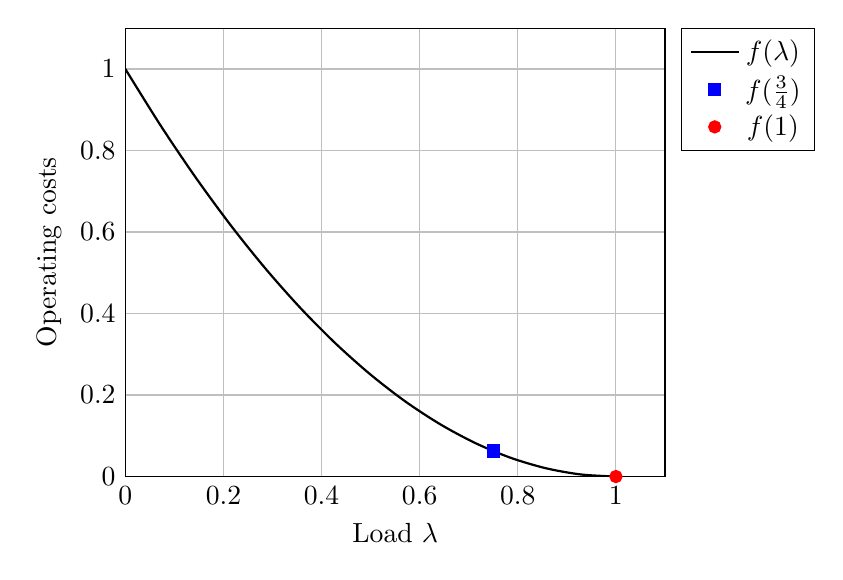
\begin{tikzpicture}
	\begin{axis}[grid=both,tick style={draw=none},every axis plot/.style={
	    domain=0:1,samples=15,smooth,thick}, 
	    xlabel=Load $\lambda$,
	    ylabel=Operating costs,
	    enlargelimits=upper,
	    legend pos=outer north east
	    ]
	\addplot[mark=none,color=black]{(x-1)^2}; 
	\addlegendentry{$f(\lambda)$};
	\addplot [only marks, mark=square*,color=blue] coordinates {(0.75,0.0625)};
	\addlegendentry{$f(\frac{3}{4})$};
	\addplot [only marks, mark=*,color=red] coordinates {(1,0)};
	\addlegendentry{$f(1)$};
	\end{axis}
\end{tikzpicture}
\end{document}
